\documentclass[25pt, a0paper,
               colspace=15mm, subcolspace=0mm,
               blockverticalspace=17mm]{tikzposter} % See Section 

\usepackage{graal-poster}
\usepackage{array}
\usepackage{multirow}
\usepackage{multicol}
\usepackage{graphicx,caption}
\usepackage{float}
\usepackage{amsmath}
\usepackage{hyperref}

\setlength{\columnsep}{2cm}


\definecolor{PaleBlue}{rgb}{0,.55,.9}
\definecolor{PaleGreen}{rgb}{0,.7,.25}
\definecolor{RedPink}{rgb}{.9,0,.2}
\definecolor{Pink}{rgb}{.85,.35,.7}
\definecolor{Purple}{rgb}{.6,0,.75}
\definecolor{Orange}{rgb}{.9,.3,.05}

\colorlet{attentionColor}{Orange}
\colorlet{charEmbedColor}{RedPink}
\colorlet{predEmbedColor}{Pink}
% \colorlet{attentionColor}{GoldUL!90!black}
% \definecolor{attentionColor}{rgb}{.85,.5,.6}

\def\pathwidth{2pt}
\def\nodewidth{3pt}
\def\cornerCurvature{7pt}

\tikzstyle{embed}=[%
  draw,
  #1,
  % line width=3pt,
  anchor=north,
  minimum width=.8cm,
  minimum height=1.6cm,
  inner sep=0pt,
  text=#1!65!black,
  font=\fontsize{25pt}{24}\selectfont,
  ]




\title{\parbox{\linewidth}{\centering Semantic segmentation for mapping hockey \\ broadcast images in 2D plan}}
\institute{Department of Computer Science and Software Engineering, Université Laval}
\author{Philippe Blouin-Leclerc\up{\dag}, Stéphane Caron\hspace{5pt}\up{\dag}}

\begin{document}
\maketitle

\begin{columns}
\column{.4}
\block{Introduction}{%
We propose a novel way to recognize key locations within hockey broadcast images using semantic segmentation and convolutional neural networks (CNN). We implement a network that learn this semantic and could then be used for many applications such as mapping a broadcast image into a 2D plan.

\vspace{5mm}
\textbf{Motivations:}
\begin{itemize}
  \item Computer vision allows the detection of many events at the same time, which is well suited for sports analytics data collection.
  \item Semantic segmentation is often a key step as it brings a \textbf{general understanding} of the image.
\end{itemize}

\vspace{5mm}
\textbf{Related work:}
\begin{itemize}
  \item Homayounfar and al. (2017): Sports field localization via deep structured models.
  \item Ronneberger and al. (2015): Convolutional networks for biomedical image segmentation (U-Net).
\end{itemize}

\vspace{0mm}
\textbf{Goals:}
\begin{itemize}
  \item Evaluate the capability of CNN to learn the semantic representation of a hockey ring surface broadcast image.
  \item Provide meaningfull insights on how to build architectures that can learn well every components of an image.
  \item Propose a method that uses semantic segmentation representation to map objects and events into a 2D plan.
\end{itemize}

% \vspace{-15pt}

}



























\column{0.6}
\block{Semantic segmentation background}{

\vspace{0mm}
Semantic segmentation is a computer vision task where the model learns the general representation of an image by attributing a label to each and every pixels.

\vspace{5mm}
\textbf{Define the task:}
In order to make pixel-wise predictions, we need to have a representation saying which class is attached to each label. This representation is what we call a \textbf{mask} (see right-side image below).

\vspace{10mm}
{\centering 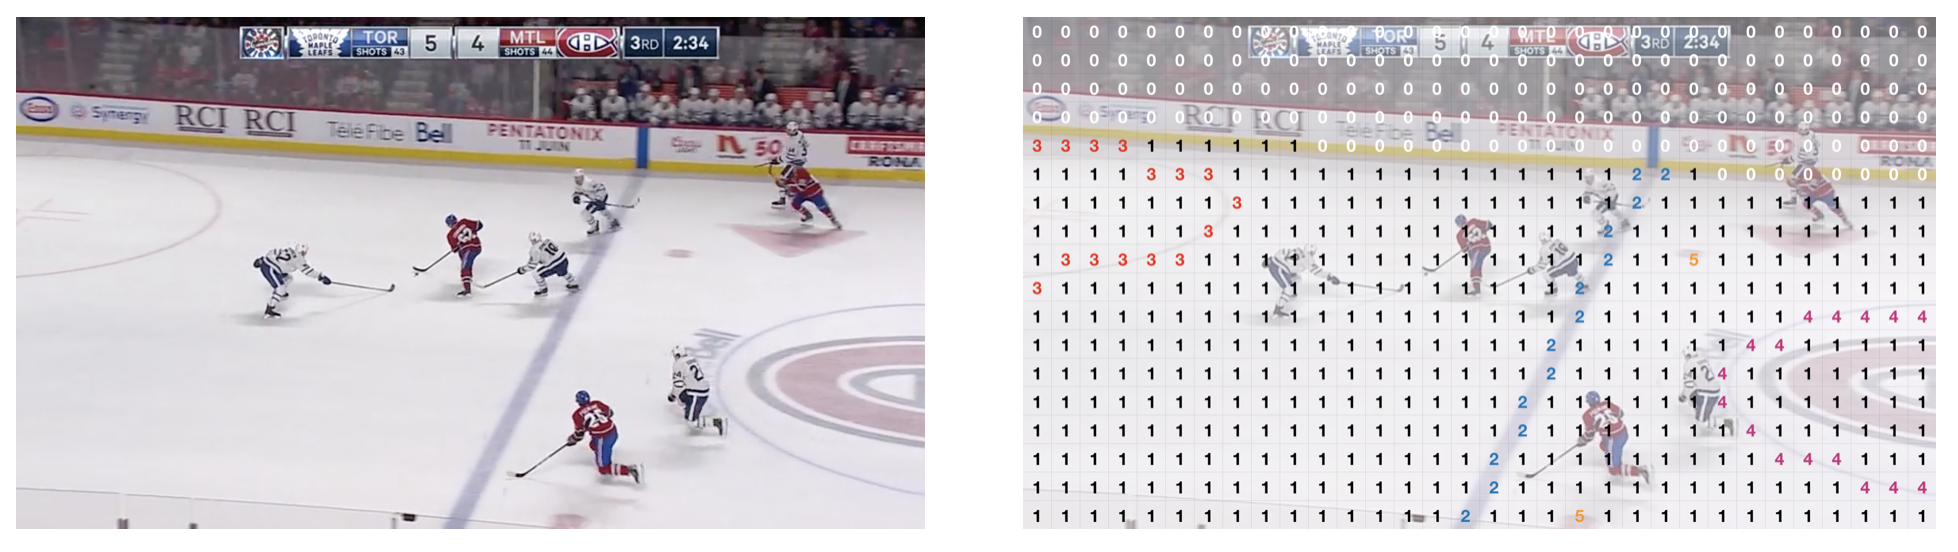
\includegraphics[width=1.0\linewidth]{figures/task-representation.png}}

As many classification problems, we need to one-hot encode all classes (one matrix for each class) which mean we can summarize the dimensions workflow as follow for one 6 classes RBG image:

\vspace{-5mm}
\begin{gather*}
	(NbChannels, Height, Width) \Rightarrow (NbLabels, Height, Width) \Rightarrow (1, Height, Width) \\
	(3, 256, 451) \Rightarrow (6, 256, 451) \Rightarrow (1, 256, 451)
\end{gather*}


}	
\end{columns}











\begin{columns}

\column{.3}


% \block[bodyoffsety=48mm, titleoffsety=48mm]{Experiments}{
\block[bodyoffsety=0mm, titleoffsety=0mm]{Methodology}{
	
Our methodology is splitted in 3 main components:

\begin{enumerate}
	\item Set up
		\begin{itemize}
			\item Dataset creation
			\item Labeling task: \href{https://github.com/opencv/cvat}{cvat tool}
		\end{itemize}
	\item Semantic segmentation
		\begin{itemize}
			\item Architecture set up
			\item Loss definition
			\item Data augmentation
			\item Training details
		\end{itemize}
	\item Mapping to 2D plan
		\begin{itemize}
			\item Key points recognition
			\item 2D translation
		\end{itemize}
\end{enumerate}


}


  \column{.7}
  \block[bodyoffsety=0mm, titleoffsety=0mm]{Architecture and training experiments}{
  	
  	\begin{multicols}{2}
  		\textbf{U-Net:} To perform our segmentation, we chose an architecture called U-Net. This network is \textbf{fast} and can be trained with \textbf{few images}.
  		
  		\vspace{10mm}
  		{\centering 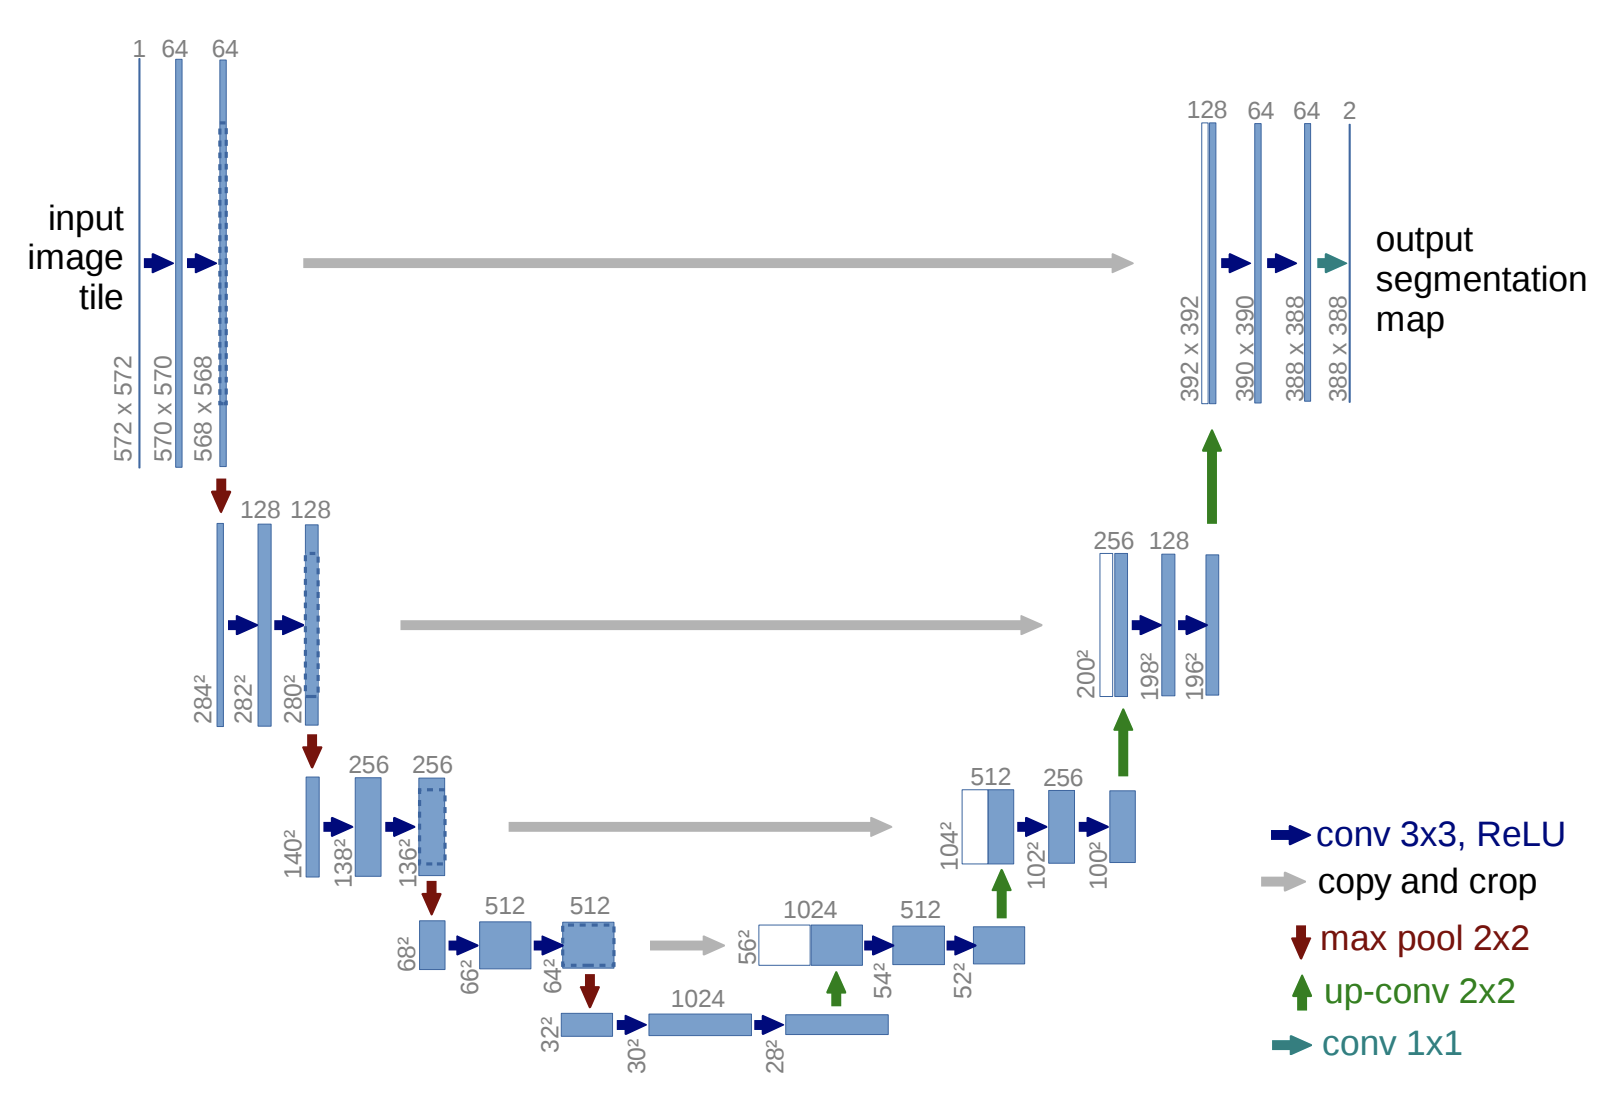
\includegraphics[width=1.0\linewidth]{figures/unet-architecture.png}}
  		
  		\columnbreak
  		
  		\textbf{Loss definition:}
  		
  		\textbf{Training details:}
  		
  	\end{multicols}
  
  
  }
  




\end{columns}




















\begin{columns}

  \column{.3}


  \block{Dataset}{

  \begin{center}
  \begin{tikzpicture}[
          scale=1.5,
          lstm_right/.style={draw, minimum width=1cm, minimum height=.5cm, inner sep=0pt, anchor=north, PaleGreen},
          lstm_left/.style={draw, minimum width=1cm, minimum height=.5cm, inner sep=0pt, PaleBlue},
          every path/.style={line width=\pathwidth},
          every node/.append style={line width=\nodewidth}]
    \def\h{2cm}
    \def\scalespace{2.2}
    \def\w{145mm}
    \def\arrowLen{.6}
    \def\descSpace{-.2}

    % Char embedding

    \foreach \word/\color/\w [count=\i] in {Salem/gray/o, Bitar/gray/o, appeared/Purple/w, to/Purple/w, have/Purple/w}{
      \pgfmathsetmacro\pos{\i-1}
      \node[anchor=mid, inner sep=0](\word) at (\scalespace*\pos,0) {\word};
      \node[embed=\color,draw=\color](\word _embed) at (\scalespace*\pos,-\arrowLen){\w};
    };

    \node[embed=black, minimum width=\w, minimum height=\h, anchor=north](comick) at ([yshift=-\arrowLen cm]appeared_embed.south) {OOV handling net};
    % \node[anchor=east, align=left] at ([xshift=\descSpace cm]comick.west) {OOV \\ handling};

    \foreach \word/\color/\w [count=\i] in {Salem/predEmbedColor/p, Bitar/predEmbedColor/p, appeared/Purple/w, to/Purple/w, have/Purple/w}{
      \pgfmathsetmacro\pos{\i-1}

      \path (\word _embed) edge[draw, -mytip] (comick.north -| \word _embed.south);
      \draw[-mytip] (comick.south -| \word _embed) -- ++(0,-\arrowLen) node[anchor=north, embed=\color, draw=\color](\word _pred_embed) {\w};

      \node[lstm_left, draw=PaleBlue, anchor=north](\word _lstm_left) at ([yshift=-\arrowLen cm]\word _pred_embed.south) {};
      \node[lstm_right, draw=PaleGreen](\word _lstm_right) at (\word _lstm_left.south) {};
      \draw[-mytip] (\word _pred_embed) -- (\word _lstm_left);
  
    };

    % LSTM arrows
    \foreach \a/\b in {Salem/Bitar, Bitar/appeared, appeared/to, to/have}{
      \draw[mytip-, PaleBlue] (\a _lstm_left) -- (\b _lstm_left);
      \draw[-mytip, PaleGreen] (\a _lstm_right) -- (\b _lstm_right);
    };
    % \node[anchor=east, align=left] at ([xshift=\descSpace cm]Salem_lstm_left.south west) {Bi-LSTM \\ task net};


    \foreach \word/\tag [count=\i] in {Salem/B-PER, Bitar/I-PER, appeared/O, to/O, have/O}{
      \pgfmathsetmacro\pos{\i-1}

      \draw[-mytip] (\word  _lstm_right.south) -- ++(0,-\arrowLen) node[embed=Orange](\word _softmax) {s};

      \node[anchor=mid, inner sep=0] (\word _tag) at ([yshift=-.5cm]\word _softmax.south) {\tag};
    };
    % \node[anchor=east, align=right] at ([xshift=\descSpace cm]Salem_tag.west) {Tags};


    % Legend
    % \begin{scope}[xshift=10.7cm, yshift=-2cm,
    \begin{scope}[xshift=-15mm, yshift=-105mm,
            every path/.style={line width=\pathwidth},
            every node/.append style={line width=\nodewidth}]
    \def\legspace{-1.3}
    \def\colsep{7}
    \def\h{1.3cm}
    % First col
    \node[embed=gray, anchor=center, minimum height=\h, minimum width=.8cm](leg char embed) at (0,0*\legspace) {o};
    \node[anchor=west] at (.5,0*\legspace) {OOV word embedding};

    \node[embed=Purple, anchor=center, minimum height=\h, minimum width=.8cm](leg word embed) at (0,1*\legspace) {w};
    \node[anchor=west] at (.5,1*\legspace) {Word embedding};

    \node[embed=predEmbedColor, anchor=center, minimum height=\h, minimum width=.8cm](leg word embed) at (0,2*\legspace) {p};
    \node[anchor=west, align=left] at (.5,2*\legspace) {Predicted embedding};


    \node[draw, PaleBlue, minimum width=1cm, inner sep=0pt, minimum height=.5cm, anchor=south] (leg lstm left) at (\colsep,0*\legspace) {};
    \node[draw, PaleGreen, minimum width=1cm, inner sep=0pt, minimum height=.5cm, anchor=north] (leg lstm right) at (leg lstm left.south) {};
    \node[anchor=west] at (\colsep+.5,0*\legspace) {Bidirectional LSTM};

    \node[embed=Orange, anchor=center, minimum height=\h, minimum width=.8cm](leg word embed) at (\colsep,1*\legspace) {s};
    \node[anchor=west, align=left] at (\colsep+.5,1*\legspace) {Tag prediction\\ with a softmax};

    \end{scope}


  \end{tikzpicture}
  \end{center}
  % \vspace{3mm}

  Two nets working together: the first predicts OOV embeddings (see OOV handling net section) and the second one predicts tags.

  The simple architecture of the labeling net is used to emphasize the usefulness of our module, and to minimize the influence of other factors.

  \vspace{-.5mm}

  }









  \column{.5}
  \block{Results}
  {
  \begin{center}
  \setlength{\tabcolsep}{5mm}
  \begin{tabular}{c c c c c c}
  \toprule
  \multirow{2}{*}{\textbf{Task}} & \multirow{2}{*}{\textbf{Tag}} & \multirow{2}{*}{\textbf{Ex.}} & \multicolumn{3}{c}{\textbf{Ponderation}}\\
  \cline{4-6}
  \addlinespace[3mm]
  & & & Word & Left & Right\\
  \midrule
  \multirow{9}{*}{NER} & O           & 1039  & \colorbold{0.81}    & 0.08    & 0.11 \\
  & B-PERS      & 63    & 0.21    & 0.31    & \colorbold{0.49} \\
  & I-PER     & 119   & 0.16  & \colorbold{0.52} & 0.32 \\
  & B-ORG     & 40  & 0.26  & 0.30  & \colorbold{0.44} \\ 
  & I-ORG     & 3     & 0.27  & 0.31      & \colorbold{0.42} \\
  & B-LOC     & 13  & 0.23      & 0.30  & \colorbold{0.47} \\
  & I-LOC     & 2     & 0.16  & \colorbold{0.48} & 0.36 \\
  & B-MISC      & 47  & \colorbold{0.40} & 0.21  & 0.39 \\
  & I-MISC      & 5     & \colorbold{0.41} & 0.26  & 0.33 \\
  \midrule
  \multirow{5}{*}{POS} & NNP  & 308 & 0.29  & 0.31  & \colorbold{0.40} \\
  & NN  & 46  & \colorbold{0.45} & 0.20  & 0.35 \\
  & CD  & 827 & \colorbold{0.86} & 0.05  & 0.09 \\
  & NNS & 23  & \colorbold{0.37} & 0.24  & \colorbold{0.39} \\
  & JJ  & 100 & \colorbold{0.49} & 0.15  & 0.36 \\
  \bottomrule
  \end{tabular}
  \end{center}
  
  \vspace{1.5mm}
   Average weights assigned to word's characters, left context and right context by the attention mechanism. We can clearly see the shift of attention according to the target entity. We also observe that the attention depends on the task at hand.
  \vspace{-3mm}
  }







  
  
  
  \column{.2}
  
%
%  \block{Performance gain}{%
%  \begin{center}
%  \setlength{\tabcolsep}{5mm}
%  \begin{tabular}{c c c c c}
%  \toprule
%  \textbf{Task} & \textbf{Metric} & \textbf{Random Emb.} & \textbf{Our module} & \textbf{Gain}\\
%  \midrule
%  NER      & F1   & 77.56 & \colorbold{80.62} & 3.9\% \\
%  POS      & acc. & 91.41 & \colorbold{92.58} & 1.2\% \\
%  % Chunking & acc. & 92.63 & 93.16  & \textbf{93.19} \\
%  % Keyphrase& F1   & 37.40 & 39.56 & \textbf{39.77} \\
%  \bottomrule
%  \end{tabular}
%  \end{center}
%  
%  \vspace{2.5mm}
%  The impact of our model on two NLP downstream tasks. We compare our OOV embeddings prediction scheme against random embeddings.
%  \vspace{-12mm}
%  }


  
  
  
  
  
  
  
  
  
  
  
  
  \block{Conclusion}{
  
  \textbf{Discussion:}
    \begin{itemize}
        \item \colorbold{Morphology} and \colorbold{context} help predict useful embeddings.
        \item \colorbold{The attention mechanism works}: depending on the task, the network will use either more the context or the morphology to generate an embedding.
    \end{itemize}
    
    \textbf{Future works:}
    \begin{itemize}
        \item  Apply the \colorbold{attention mechanism on each character of the OOV word and each word of the context} instead of using the hidden state of the respective elements only.
        \item Test our attention model in \colorbold{different languages} and on other NLP tasks, such as \colorbold{machine translation}.
    \end{itemize}
    \vspace{-3.5mm}
  }
\end{columns}

\end{document}